In the framework of advanced, active hand prosthetics, nowadays we are
witnessing a sort of technology transfer from robotics and
mechatronics. Touch Bionics's i-LIMB \cite{ilimb} prosthetic hand,
with its five degrees-of-freedom, is a real breakthrough with respect
to the previous state-of-the-art, Otto Bock's SensorHand Speed
\cite{sensorhand}, which is essentially an open-close
mechanism. Dexterity of hand prostheses is still far from that of
state-of-the-art non-prosthetic mechanical hands, such as, e.g., the
DLR II \cite{Hua2006} (not to mention a human hand, of course), but
things are getting better thanks to the aforementioned
inter-disciplinary exchange (see Figure \ref{fig:hands}). Several
EU-funded projects (e.g., CyberHand \cite{CyberHand} and SmartHand
\cite{smarthand}) testify the enthusiasm in the field.

\begin{figure}
  \begin{tabular}{ccc}
    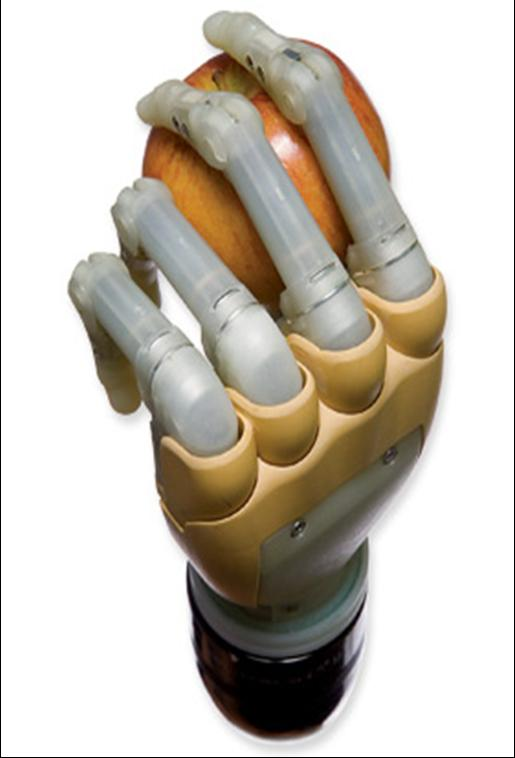
\includegraphics[width=0.14\textwidth]{figs/hands_TB.jpg} &
    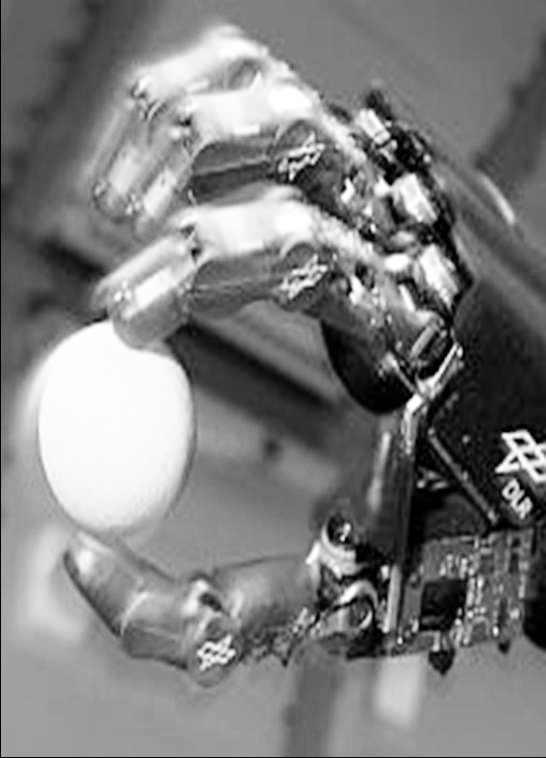
\includegraphics[width=0.14\textwidth]{figs/hands_DLRII.jpg} &
    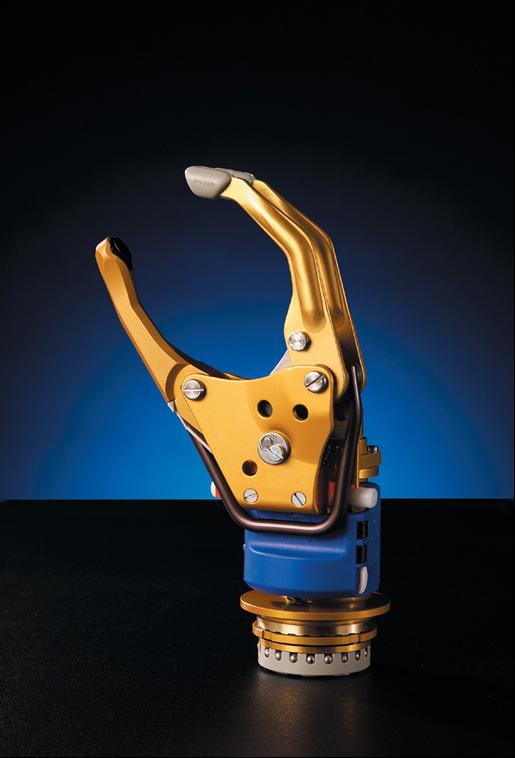
\includegraphics[width=0.14\textwidth]{figs/hands_OB.jpg} \\
    $(a)$ & $(b)$ & $(c)$
  \end{tabular}
  \caption{$(a)$ Touch Bionics's i-LIMB prosthetic hand (reproduced
    from \cite{ilimb}); $(b)$ the DLR-II mechanical hand; $(c)$ Otto
    Bock's SensorHand Speed (reproduced from \cite{sensorhand}).}
  \label{fig:hands}
\end{figure}

The simplest, cheapest and therefore most used technique for
interfacing the patient with the prosthesis is surface
electromyography (EMG): activation potentials of the patient's stump
residual muscles are detected to move the hand to predefined
positions. But the control schema employed is rather poor, using two
or three electrodes to issue an ``open/close'' command or, in the more
advanced case of the i-LIMB, to choose among a predefined set of grasp
shapes.
%% The electrodes are associated with large muscles in the
%% patient's stump, such as, e.g., the wrist flexor and extensor. The
%% result is a highly non-natural form of control, e.g., wrist flexion
%% corresponding to opening, and there is no chance of controlling the
%% desired force. The patient must, in turn, learn how to activate the
%% residual muscles to control the prosthesis

%% A general sense of frustration impends, as far as control is
%% concerned. How is an amputee supposed to \emph{naturally} command the
%% prosthesis what to do (i.e., how to grasp an object) and with what
%% force?

In order to control the prosthesis in a more natural way, machine
learning can be used to better interpret the standard EMG signals. In
the typical case, the patient is asked to imagine, e.g., a pinch grip;
the related EMG pattern is then used to obtain a pinch grip with the
required force from the prosthesis. A degree of control unknown so far
can be thus obtained, improving the patient's life and shortening the
training time. We envision \emph{adaptive prosthetics}, a framework in
which a patient enters a virtuous loop of \emph{reciprocal learning},
whereas so far (s)he has to learn how to control the prosthesis from
scratch.

%% A
%% final very agreeable point is that standard, commercially available
%% EMG electrodes can be used to this end.
%% 
%% The idea is that of improving the patient's quality of life by
%% providing an \emph{adaptive prosthesis}, so that he/she enters a
%% virtuous loop of \emph{reciprocal learning}, whereas so far the
%% patient has to learn how to control the prosthesis from scratch.

To further improve this loop it is desirable to \emph{pre-train} the
prosthesis with a model which will be then refined and adapted on-line
to the patient. In machine learning, this is called \emph{model
adaptation}: a system which adapts to a new data distribution, as this
distribution shifts with time. Model adaptation in this framework
works like this: \textbf{FRANCESCO: brevissimo riassunto dell'approccio}

To check whether this idea can improve things, we apply it to a set of
EMG data collected from $10$ healthy subjects. Each subject was asked
to grasp a force sensor in different conditions and using three
different grips. Meanwhile, we recorded the electrical activity of the
muscles that are most involved in the hand/wrist movements and the
force exerted by the subject on a off-the-shelf force sensor. The
experimental results show that our intuition is correct, to the point
that \textbf{FRANCESCO: riassunto dei risultati}.

The paper is structured as follows: after a brief review of related
work, 
%we clearly state the problem we want to solve (Section
%\ref{sec:prob}); then, 
we describe our method (
Section \ref{sec:math}) and the EMG database (Section \ref{sec:mms}) %give
%detail about our method and the EMG database. 
Section \ref{sec:exp}
shows the experimental results and lastly Section \ref{sec:concl}
contains the conclusions.

\subsection{Related Work}

The use of surface forearm EMG to control active hand prostheses dates
back to the Fifties and was brought to the market by Otto Bock
Orthopaedic Industry, Inc. \cite{history}. EMG works by detecting a
muscle's activation potential, a fast oscillating signal whose
root-mean-square is non-linearly related to the force exterted by the
muscle \cite{deluca}. Since amputees are usually left with little of
their forearm, it has so far been necessary to carefully detect the
patient's residual muscles with the strongest activity. These muscles
are used, still nowadays, to control one, or at best two
degrees-of-freedom. For example, the usual control schema of Otto
Bock's SensorHand Speed prosthetic hand maps wrist flexion to hand
closing and wrist extension to hand opening.

The situation hasn't changed for a long time because the EMG signal is
badly conditioned, being influenced by sweat, muscular fatigue,
inter-arm differences and non-hand-related muscular activity
(supination/pronation, walking, raising one's arms and so on; see
\cite{zecca} for a survey). Only in the 1990s it became apparent that
machine learning could be used to classify hand postures via the
EMG. In their seminal work, Bitzer and van der Smagt \cite{smagt}
could use a Support Vector Machine to robustly classify six different
hand postures. Neural networks and LWPR \cite{lwpr} have been used to
the same end (see, e.g., \cite{2008.ICRA,2008.BioCyb,Sebelius2005}) to
classify up to $11$ hand/finger postures and movements, and to
approximate the force involved in the grasp. As long as it is trained
for a sufficient time, that is it explores a relevant portion of the
input space, a well-employed machine learning method will be able to
take into account all of the EMG signal's problems.

As far as we know, there is no EMG database present in the machine
learning community, which could serve our purpose. In some of the
aforementioned papers, analogous data sets (but most likely smaller
than ours) are reported about, but there is no mention of their
availability. 
%The data set used in this paper has been gathered in
%2008 and is the subject of another analysis whose preliminary results
%are visible in \cite{2008.GNB}. A larger, full report is being
%prepared for submission.
%FIXME CLAUDIO: mi sembra inutile e potenzialmente dannoso (se il db non e' nuovo, e un contributo di meno del paper), lo toglierei 
\textbf{FRANCESCO: model adaptation in letteratura...}

